\documentclass[12pt]{article}
\usepackage{authblk}
\usepackage{upgreek}
\usepackage{multirow}
\usepackage{indentfirst}
\usepackage{setspace}
\usepackage{geometry}
\usepackage{graphicx}
\usepackage{newtxtext, newtxmath}
\geometry{a4paper,left=2.45cm,right=2.45cm,top=2.45cm,bottom=2.45cm}
\title{\huge Design and Analysis of a Laminated Composite Tube}
\author{Jiatai Deng, Jiawei Shuang, Xuanye Hu}
\affil{Department of Mechanical, Aerospace and Civil Engineering}
\date{\today}
\newpage
\begin{document}
\newpage
\maketitle
\thispagestyle{empty}
\newpage
\tableofcontents
\thispagestyle{empty} 
\newpage

\section{General description and requirement}
\setcounter{page}{1}
\pagenumbering{arabic}
\onehalfspacing
\noindent A cylindrical tube of 4 layers of composite with a layup of 
$\left[\alpha\  \beta\  \alpha\  \beta\right]$
is to be designed and by winding tapes cut from a UD carbon-epoxy prepreg sheet on to a cylindrical mandrel of a 25mm radius. For the consideration of practicality, the range of these two winding angles will have to fall in [-75°, -30°] or [+30°, +75°] to the axis of the tube. The thickness of the prepreg is 0.25mm. The tube should be made to a length of 300mm.  \newline
\noindent \textbf{Material properties:}\newline
Internal pressure: $q = 3\times10^{6}$ \qquad Axial force: $P = 25 kN$ \newline
Tube radius: $R = 25\times10^{-3}$ \qquad  Tube length $L = 0.3$ \newline
Elastic constant: $E1 = 236 GPa$ \qquad $E2 = 5 GPa$ \qquad $G = 2.6 GPa$ \qquad $\upsilon_{12} = 0.25 GPa$ \newline
Strengths: $\sigma_{1t}^{*} = 3800 MPa$ \qquad $\sigma_{2t}^{*} = 41 MPa$ \qquad $\sigma_{1c}^{*} = 689 MPa$ \qquad $\sigma_{2c}^{*} = 107 MPa$\qquad\qquad\qquad $\tau _{12}^{*} = 69 MPa$ 
\section{Design approach and theory}
• Composite tube is a laminated structure
• A developed tube is a laminate ‒ Lay up: $[\alpha /\beta /\alpha /\beta ]$
• Laminate theory can be used for stress analysis
\newline
\noindent STEP I: Define the two winding angles:\newline
\begin{center}
$-75^{\circ} \leq \alpha \leq -30^{\circ}$ or $75^{\circ} \leq \alpha \leq 30^{\circ}$\end{center}
\begin{center}
$-75^{\circ} \leq \beta \leq -30^{\circ}$ or $75^{\circ} \leq \beta \leq 30^{\circ}$
\end{center}
\noindent STEP II: Define the Stress-Strain Relationship $\left[ Q \right]$:\newline
According to the Laminar Stress-Strain Relationship in Material coordinate system: \newline$$\left\{ \sigma \right\} = \left[Q \right] \left\{ \epsilon \right\}$$
$$\left\{ \begin{matrix}
    \sigma_1  \\
    \sigma_2  \\
    \tau_{12}  \\
    \end{matrix} \right\} = \left[\begin{matrix}
		Q_{11} & Q_{12} & 0 \\
		Q_{12} & Q_{22} & 0 \\
		0 & 0 & Q_{66} \\
		\end{matrix} \right] \left\{ \begin{matrix}
			\epsilon_1  \\
			\epsilon_2  \\
			\gamma_{12}  \\
			\end{matrix} \right\} = \left[\begin{matrix}
				\frac{E1}{1-\upsilon^2\frac{E2}{E1}} & \frac{\Upsilon E2}{1-\upsilon^2\frac{E2}{E1}} & 0 \\
				\frac{\Upsilon E2}{1-\upsilon^2\frac{E2}{E1}} & \frac{E2}{1-\upsilon^2\frac{E2}{E1}} & 0 \\
				0 & 0 & G \\
				\end{matrix} \right] \left\{ \begin{matrix}
					\epsilon_1  \\
					\epsilon_2  \\
					\gamma_{12}  \\
					\end{matrix} \right\}$$
\noindent STEP III: Define the Coordinate transformation $\left[ T \right]$
\noindent The winding angle of 4 layers of composite: $ \theta = \left( \begin{matrix}
	\alpha  \\
	\beta  \\
	\alpha  \\
	\beta	\\
	\end{matrix} \right)$, the coordinate transformation between (x-y) and (1-2) matrix:$$ \left\{ T \right\} = \left[\begin{matrix}
			\cos^2{\theta} & \sin^2{\theta} & -2\cos{\theta}\sin{\theta} \\
			\sin^2{\theta} & \cos^2{\theta} & 2\cos{\theta}\sin{\theta} \\
			\cos{\theta}\sin{\theta} & -\cos{\theta}\sin{\theta} & cos^2{\theta}-sin^2{\theta} \\
			\end{matrix} \right]$$\newline

\noindent STEP IV: Define maximum stress failare criterion\newline
According to the maximum stress failure criterion, material will fail when any of the following conditions is violated:\newline
$$\frac{\sigma_1}{\sigma^*_{1t}} \leq 1 \quad if \quad \sigma_1 > 0 \qquad\qquad\qquad \frac{\left| \sigma_1 \right|}{\sigma^*_{1c}} \leq 1 \quad if \quad  \sigma_1 < 0$$
$$\frac{\sigma_2}{\sigma^*_{2t}} \leq 1 \quad if \quad \sigma_2 > 0 \qquad\qquad\qquad \frac{\left| \sigma_2 \right|}{\sigma^*_{2c}} \leq 1 \quad if \quad  \sigma_2 < 0$$
$$\frac{\left| \tau_{12} \right|}{\tau^*_{12}} \leq 1$$\newline\newline
\noindent STEP V: Define Twist angle
Tube is fixed at the bottom end and axially compressed at the top.
Generator on the tube deforms by an angle $\gamma_{xy}$.
Point $A$ at the top end moves to $A′$ by a distance $\gamma_{xy}L$.
We can get the twist angle of the tube formula:\newline
\begin{minipage}[b]{0.7\linewidth}
	$$\theta = \frac{\gamma_{xy}L}{R}$$\newline\newline
	\end{minipage}
	\hfill
	\begin{minipage}[b]{0.3\linewidth}
		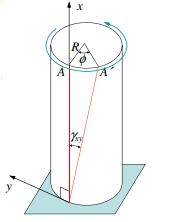
\includegraphics{twist.png}
	\end{minipage}
\noindent\textbf{There are two loading conditions, separately analysis:}
\subsection{Case 1}
\noindent Internal pressure of 3 MPa (ends closed)\newline
\begin{minipage}[b]{0.7\linewidth}
The generalised stresses:
	$ \left\{ \begin{matrix}
		N_x=\frac{1}{2}qR \\
		N_y=qR\newline  \\
		N_{xy}=0 
		\right\ }  \\
		\end{matrix} \right\}$
	\end{minipage}
	\hfill
	\begin{minipage}[b]{0.3\linewidth}
	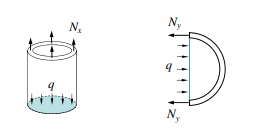
\includegraphics{case1.png}
	\end{minipage}

\noindent 
\subsection{Case 2}
\noindent Apply Axial compression of $P = 25 kN$\newline
\begin{minipage}[b]{0.7\linewidth}
The generalised stresses:
	
\section{ Results and analysis to prove the success of the design }
\noindent With 
\section{steering mechanism}
\noindent In 
\section{Appendix}
\textbf{Matlab code}
\begin{lstlisting}
%%Unit: Pa,m%%
%%Term CASE1FM loading case 1 Failure matrix%%
%%Term CASE2FM loading case 2 Failure matrix%%
%%Term AssemblyFM Assembled Falure matrix [-30,30] has been removed%%
%%Term CASE2TA loading case 2 twist angle%%
%%Term BP Best point%%

format short %%Modify according to the requirement%%

%%Basic parameters%%

resolution=1; %%Modify according to the requirement%%
Delete=[0]; %%leave it alone%%
q=3e6;
P=-2.5e4;
R=25e-3; 
thick=2.5e-4;
L=0.3;
E1=236e9;
E2=5e9;
G=2.6e9;
v=0.25;
Xt=3800e6;
Xc=689e6;
Yt=41e6;
Yc=107e6;
S=69e6;
TAT_1=zeros(150/resolution+1); %%Initial matrix of Twist Angle%%
TAT_1=zeros(150/resolution+1);
for i=-75/resolution:1:75/resolution %%2 for loots control the Alpha and Beta%%
	Alpha=i*resolution;
	AlphaF=i+75/resolution+1;
	for i=-75/resolution:1:75/resolution
		Beta=i*resolution;
		BetaF=i+75/resolution+1;
		Theta=[Alpha;Beta;Alpha;Beta];
		t=[thick;thick;thick;thick];
		ctraQ=1-((v^2)*(E2/E1));
		Q=[E1/ctraQ v*E2/ctraQ 0; v*E2/ctraQ E2/ctraQ 0; 0 0 G];
		TT=[0;0;0];
			for i = 1:4 %%Find related equition in sheet%%
				straTAlpha=sind(Theta(i));
				ctraTAlpha=cosd(Theta(i));
				TAlpha=[ctraTAlpha^2 straTAlpha^2 -2*ctraTAlpha*straTAlpha;
				straTAlpha^2 ctraTAlpha^2 2*ctraTAlpha*straTAlpha;
				ctraTAlpha*straTAlpha -ctraTAlpha*straTAlpha ctraTAlpha^2-straTAlpha^2];
				TT=[TT TAlpha];
				eval(['TT',num2str(i),'=TAlpha;'])
			end
		TT=TT(:, 2:13);
		A=zeros(3);
			for i=1:4
				m=(i-1)*3+1;
				n=i*3;
				TTa=TT(:,m:n);
				A=A+thick*TTa*Q*TTa';
				Delete=Delete';
			end
		a=A^(-1);
		Q0=Q;

		%%Case one%%

		N_1=[0.5*q*R; q*R; 0];
		Epsilonx_1=a*N_1;
		Phi_1=Epsilonx_1(3)*L/R*180/pi;
		TAT1(AlphaF,BetaF)=Phi_1;
			for i=1:4
				m=(i-1)*3+1;
				n=i*3;
				TTa=TT(:,m:n);
				Epsilon_1= TTa'*Epsilonx_1;
				Delete=Delete';
				Sigma=Q0*Epsilon_1;
					if Sigma(1)>=0
						w1=Sigma(1)/Xt;
					else 
						w1=-Sigma(1)/Xc;
					end
					if Sigma(2)>=0
						w2=Sigma(2)/Yt;
					else
						w2=-Sigma(2)/Yc;	
					end
				w3=abs(Sigma(3)/S);
				w=[w1; w2; w3];
				eval(['wcone',num2str(i),'=w;'])
			end
		wwassembly_1=[wcone1 wcone2 wcone3 wcone4];	
		Fail_case_one_1=all(wwassembly_1(:)<=1);
		TATT_1(AlphaF,BetaF)=Fail_case_one_1;
		TATT_1=TATT_1*1;

		%%Case two%%

		N_2=[P/(2*pi*R); 0; 0];
		Epsilonx_2=a*N_2;
		Phi_2=Epsilonx_2(3)*L/R*180/pi;
		TAT_2(AlphaF,BetaF)=Phi_2;
			for i=1:4
				m=(i-1)*3+1;
				n=i*3;
				TTa=TT(:,m:n);
				Epsilon_2= TTa'*Epsilonx_2;
				Delete=Delete';
				Sigma=Q0*Epsilon_2;
					if Sigma(1)>=0
						w1=Sigma(1)/Xt;
					else 
						w1=-Sigma(1)/Xc;
					end
					if Sigma(2)>=0
						w2=Sigma(2)/Yt;
					else
						w2=-Sigma(2)/Yc;
					end
				w3=abs(Sigma(3)/S);
				w=[w1; w2; w3];
				eval(['wcone',num2str(i),'=w;'])
			end
		wwassembly_2=[wcone1 wcone2 wcone3 wcone4];
		Fail_case_one_2=all(wwassembly_2(:)<=1);
		TATT_2(AlphaF,BetaF)=Fail_case_one_2;
		TATT_2=TATT_2*1;
	end
end

CASE1FM=TATT_1;
XX=-75:resolution:75;
YY=-75:resolution:75;
CASE2FM=TATT_2;
CASE2TA=TAT_2;
CASE1FM((-30+75)/resolution+1:(30+75)/resolution+1,:)=0;
CASE1FM(:,(-30+75)/resolution+1:(30+75)/resolution+1)=0;

CASE2FM((-30+75)/resolution+1:(30+75)/resolution+1,:)=0;
CASE2FM(:,(-30+75)/resolution+1:(30+75)/resolution+1)=0;

%%Assemble the Failure matrix%%

AssemblyFM=CASE1FM.*CASE2FM;

%%Find the best point%%

TAFM=AssemblyFM.*CASE2TA;
BPZ=max(max(TAFM));
[BPX BPY]=find(TAFM==max(max(TAFM)));
BPX=(BPX(1)-1-75/resolution)*resolution;
BPY=(BPY(1)-1-75/resolution)*resolution;
BP=[BPX BPY BPZ]

%%0 become NAN for figure%%

ind=find(TAFM==0);  
TAFM(ind)=NaN;

%%Figure%%
	%%Colormap transformation%%

colormap(parula);

	%%TA Figure%%

mesh(XX,YY,CASE2TA);
title('Twist Angle','Fontname', 'Times New Roman','FontSize',24);
x1=xlabel('Alpha (degree)','Fontname', 'Times New Roman','FontSize',18);
x2=ylabel('Beta (degree)','Fontname', 'Times New Roman','FontSize',18);
x3=zlabel('Twist angle (degree)','Fontname', 'Times New Roman','FontSize',18);
set(x1,'Rotation',18);
set(x2,'Rotation',-25);

saveas(gcf,'Twist Angle.jpg');

	%%TA plane figure%%

contour(XX,YY,CASE2TA,10,'ShowText','on');
title('Twist Angle (degree)','Fontname', 'Times New Roman','FontSize',24);
x1=xlabel('Alpha (degree)','Fontname', 'Times New Roman','FontSize',18);
x2=ylabel('Beta (degree)','Fontname', 'Times New Roman','FontSize',18);

saveas(gcf,'Twist Angle (degree).jpg');

	%%TA Figure without Failure%%

mesh(XX,YY,TAFM);
title('Twist Angle without Failure','Fontname', 'Times New Roman','FontSize',24);
x1=xlabel('Alpha (degree)','Fontname', 'Times New Roman','FontSize',18);
x2=ylabel('Beta (degree)','Fontname', 'Times New Roman','FontSize',18);
x3=zlabel('Twist angle (degree)','Fontname', 'Times New Roman','FontSize',18);
set(x1,'Rotation',18);
set(x2,'Rotation',-25);

saveas(gcf,'Twist Angle without Failure.jpg');

	%%Colormap transformation%%

colormap(gray);

	%%Devided failure analysis figure%%

gca=pcolor(XX,YY,CASE1FM);
set(gca, 'LineStyle','none');
title('Failure Analysis of Case One','Fontname', 'Times New Roman','FontSize',24);
x1=xlabel('Alpha (degree)','Fontname', 'Times New Roman','FontSize',18);
x2=ylabel('Beta (degree)','Fontname', 'Times New Roman','FontSize',18);

saveas(gcf,'Failure Analysis of Case One.jpg');

gca=pcolor(XX,YY,CASE2FM);
set(gca, 'LineStyle','none');
title('Failure Analysis of Case Two','Fontname', 'Times New Roman','FontSize',24);
x1=xlabel('Alpha (degree)','Fontname', 'Times New Roman','FontSize',18);
x2=ylabel('Beta (degree)','Fontname', 'Times New Roman','FontSize',18);

saveas(gcf,'Failure Analysis of Case Two.jpg');

	%%Assembled failure analysis figure%%

gca=pcolor(XX,YY,AssemblyFM);
set(gca, 'LineStyle','none');
title('Failure Analysis','Fontname', 'Times New Roman','FontSize',24);
x1=xlabel('Alpha (degree)','Fontname', 'Times New Roman','FontSize',18);
x2=ylabel('Beta (degree)','Fontname', 'Times New Roman','FontSize',18);

saveas(gcf,'Failure Analysis.jpg');
	\end{lstlisting}

\begin{itemize}
	\item[-] Design for jump demonstration:
	Add basic moving features to increase the range of activities.
	\item[-] Design for jump demonstration:
	Add basic moving features to increase the range of activities.
	\item [-] Design within the limits of printed parts resistance:
	Increase overall structural strength to prevent failures from occurring.
	\item [-] Untethered design:
	if there are other ideas and optimizations, they could also be discussed too.
\end{itemize}

\end{document}
\begin{thebibliography}{widestlabel}
	\bibitem{ref1}Hale, E., Schara, N., Burdick, J. and Fiorini, P., 2000, April. A minimally actuated hopping rover for exploration of celestial bodies. In Proceedings 2000 ICRA. Millennium Conference. IEEE International Conference on Robotics and Automation. Symposia Proceedings (Cat. No. 00CH37065) (Vol. 1, pp. 420-427). IEEE.
\end{thebibliography}{99}  
  
